\vspace{10pt}

{\centering\subsection*{刘笑:游花海}}

\addcontentsline{toc}{subsection}{刘笑:游花海}

\renewcommand{\leftmark}{刘笑:游花海}

\begin{figure}[htbp]

\centering

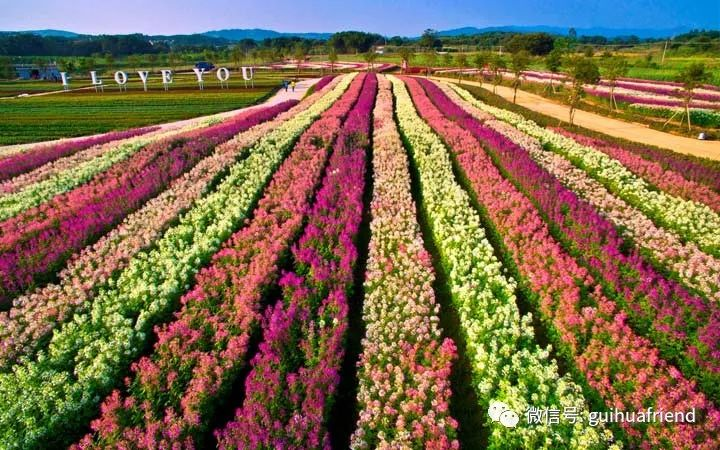
\includegraphics[width = .5\textwidth]{./ch/6.jpg}

\end{figure}





你们在日常生活中游览过哪些地方呢?在你的印象中,最深刻的是什么呢?就让我来说说我印象中最深刻的一件事吧!我印象中最深刻的是游花海。

今天妈妈要带我和弟弟去花海玩,那里的花争奇斗艳,芬芳迷人。

我们先从南门进去,往西走就来到了一片美丽的玫瑰花园,那里的玫瑰有好几种颜色,漂亮极了,红色的玫瑰花像是铺了一条红色的地毯。当微风吹过时,它们摇摇头,仿佛是在说我美丽吗?你多看看我吧!

在玫瑰花园的北面就到了向日葵园。那里的向日葵有的高,有的低。往上看,仿佛是弯弯曲曲的山坡。如果你从远处望去,那就仿佛是一个个又大又圆的太阳。那向日葵中间还有很多很多瓜子。

向日葵的西边是一个小亭子,站在那里往东望去,就是用各色的玫瑰花摆成的一个爱心,旁边还有许多小风筝摆的一些字母。

这就是我想和你们说的印象中最深刻的事。你们也和我说说在你印象中最深刻的一件事吧!





\vspace{10pt}



作者:四(2)班 刘笑



指导老师:陈小丽



投稿:2021年6月9日



发表:2021年6月10日














                



\vspace{10pt}

\hline



